\documentclass[conference]{IEEEtran}
\usepackage{graphicx}
\usepackage{amsmath}
\usepackage{cite}
\usepackage{hyperref}
\usepackage{float}

\title{Interaction Between a Single Quantum Emitter and a Single-Mode Cavity}
\author{\IEEEauthorblockN{Ziyu Zhou}
\IEEEauthorblockA{
Department of Electrical and Computer Engineering\\
Rice University, Houston, TX, USA\\
Email: zz107@rice.edu}
}

\begin{document}

\maketitle

\begin{abstract}
This study investigates the interaction between a single quantum emitter (T center) and a single-mode cavity using the Jaynes-Cummings model. The analysis focuses on Vacuum Rabi oscillations under varying coupling strengths, dissipation rates, and thermal noise levels. By solving the master equation numerically, we explore how these parameters influence the quantum dynamics. The results are analyzed using the Python QuTiP library, providing insight into potential applications in quantum communication and scalable quantum networks.
\end{abstract}

\section{Introduction}

Cavity quantum electrodynamics (Cavity QED) is a subfield of quantum optics that examines the interaction between quantum emitters and confined electromagnetic fields in optical or microwave cavities. These systems provide a platform for studying quantum phenomena such as coherent energy exchange, entanglement generation, and quantum state transfer.

\subsection{Strong Coupling Regime in Cavity QED}
The strong coupling regime is a critical condition in Cavity QED, characterized by a coupling strength $g$ between the quantum emitter and the cavity mode that exceeds the dissipation rates of the system ($\kappa$ for the cavity and $\gamma$ for the emitter). This regime enables coherent energy exchange, manifesting as **Vacuum Rabi oscillations**, where energy oscillates between the emitter and the cavity mode.

Experiments with superconducting qubits and photonic crystals have successfully demonstrated strong coupling. Superconducting qubits embedded in microwave cavities serve as a platform for scalable quantum computing. Photonic crystal cavities, on the other hand, leverage subwavelength confinement of light, achieving high $Q$-factors and small mode volumes.

\subsection{Hybrid Quantum Systems}
Hybrid systems combine solid state defects (e.g. nitrogen vacancy centers, T centers) with optical cavities. These systems enable efficient photon emission and quantum state storage, making them essential for quantum networks. For example, T centers embedded in silicon provide long coherence times and compatibility with existing silicon photonics infrastructure.

\subsection{Advanced Cavity Designs}
Cavity designs such as photonic crystal cavities and Fabry-Pérot cavities have been optimized to minimize dissipation. High $Q$-factor photonic crystal cavities achieve ultra-low loss, enabling long coherence times crucial for quantum error correction and robust quantum operations.

\subsection{Theoretical Background}
The Jaynes-Cummings model describes the interaction between a two-level emitter and a single-cavity mode. The system Hamiltonian is expressed as:
\begin{equation}
H = \hbar \omega_c a^\dagger a + \hbar \omega_a \sigma^+ \sigma^- + \hbar g \left(a^\dagger \sigma^- + a \sigma^+\right),
\end{equation}
where:
\begin{itemize}
    \item $\omega_c$: Cavity frequency.
    \item $\omega_a$: Emitter frequency.
    \item $g$: Coupling strength.
    \item $a^\dagger$, $a$: Creation and annihilation operators for the cavity mode.
    \item $\sigma^+$, $\sigma^-$: Raising and lowering operators for the emitter.
\end{itemize}

The system's dynamics, including dissipation and thermal noise, are modeled using the Lindblad master equation:
\begin{equation}
\frac{d\rho}{dt} = -\frac{i}{\hbar}[H, \rho] + \sum_i \mathcal{D}[C_i]\rho,
\end{equation}
where $\mathcal{D}[C_i]\rho = C_i \rho C_i^\dagger - \frac{1}{2}\{C_i^\dagger C_i, \rho\}$ represents dissipative processes.

\section{Methods}

\subsection{Numerical Simulation with QuTiP}
The dynamics of the quantum emitter-cavity system are simulated using Python’s QuTiP library. The simulation workflow includes defining the system’s Hamiltonian, dissipation processes, initial state, and solving the master equation.

\subsubsection{Defining the System Operators}
The annihilation operator for the cavity and lowering operator for the emitter are defined as:
\begin{equation}
a = \texttt{destroy(N)}, \quad \sigma^- = \texttt{destroy(2)},
\end{equation}
where $N$ is the number of Fock states representing the cavity mode.

\subsubsection{Constructing the Hamiltonian}
The Hamiltonian is implemented in QuTiP as:

\texttt{H = wc * a.dag() * a + wa * sm.dag() * sm + g * (a.dag() * sm + a * sm.dag())}

where $wc$, $wa$, and $g$ represent the cavity frequency, emitter frequency, and coupling strength.

\subsubsection{Adding Dissipation}
Dissipative effects are included using Lindblad operators:
\begin{itemize}
    \item \textbf{Cavity Dissipation}:
    \begin{equation}
    C_{\text{cavity}} = \sqrt{\kappa(1 + n_{th})}a, \quad C_{\text{cavity}}^\dagger = \sqrt{\kappa n_{th}}a^\dagger
    \end{equation}
    \item \textbf{Emitter Decay}:
    \begin{equation}
    C_{\text{emitter}} = \sqrt{\gamma}\sigma^-
    \end{equation}
\end{itemize}
These are implemented in QuTiP as:
{\scriptsize
\begin{verbatim}
c_ops.append(np.sqrt(kappa * (1 + n_th)) * a)
c_ops.append(np.sqrt(kappa * n_th) * a.dag())
c_ops.append(np.sqrt(gamma) * sm)
\end{verbatim}
}

\subsubsection{Defining the Initial State}
The initial state of the system is:
\begin{equation}
|\psi(0)\rangle = |0\rangle_{\text{cavity}} \otimes |1\rangle_{\text{emitter}},
\end{equation}
defined in QuTiP as:
\begin{verbatim}
psi0 = tensor(basis(N, 0), basis(2, 1))
\end{verbatim}

\subsection{Solving the Master Equation}
The system's time evolution is computed using \texttt{mesolve}:
{\scriptsize
\begin{verbatim}
output = mesolve(H, psi0, tlist, c_ops, observables)
\end{verbatim}
}
Here, \texttt{observables} represents the operators $\langle a^\dagger a \rangle$ and $\langle \sigma^+ \sigma^- \rangle$, corresponding to the cavity photon number and emitter population.


\subsection{Parameter Exploration}
Simulations are performed by varying:
\begin{itemize}
    \item Coupling strength ($g$): From 0.1 to 2.
    \item Dissipation rates ($\kappa$, $\gamma$): From 0.001 to 0.1.
    \item Thermal noise ($n_{th}$): From 0 to 2.
\end{itemize}


\section{Results}

This section presents the results of numerical simulations analyzing the quantum emitter-cavity system under various conditions, focusing on vacuum Rabi oscillations, dissipation rates, and thermal noise.

\subsection{Vacuum Rabi Oscillations for Different Coupling Strengths}

Figure~\ref{fig:coupling_strength} illustrates the vacuum Rabi oscillations for varying coupling strengths ($g$). At $g = 0$, there is no energy exchange between the emitter and cavity. Increasing $g$ enhances the oscillation frequency and amplitude, showcasing stronger coherence at higher coupling strengths.

\begin{figure}[h!]
    \centering
    \includegraphics[width=0.8\linewidth]{1.png}
    \caption{Vacuum Rabi Oscillations for different coupling strengths ($g$). The values of $g$ range from 0 to 1.0.}
    \label{fig:coupling_strength}
\end{figure}

\subsection{Oscillation Frequency and Decay Rate vs. Coupling Strength}

The relationship between coupling strength and oscillatory properties is presented in Figure~\ref{fig:frequency_decay}. The left panel demonstrates a linear increase in oscillation frequency with $g$, while the right panel shows the decay rate stabilizing at higher coupling strengths.

\begin{figure}[h!]
    \centering
    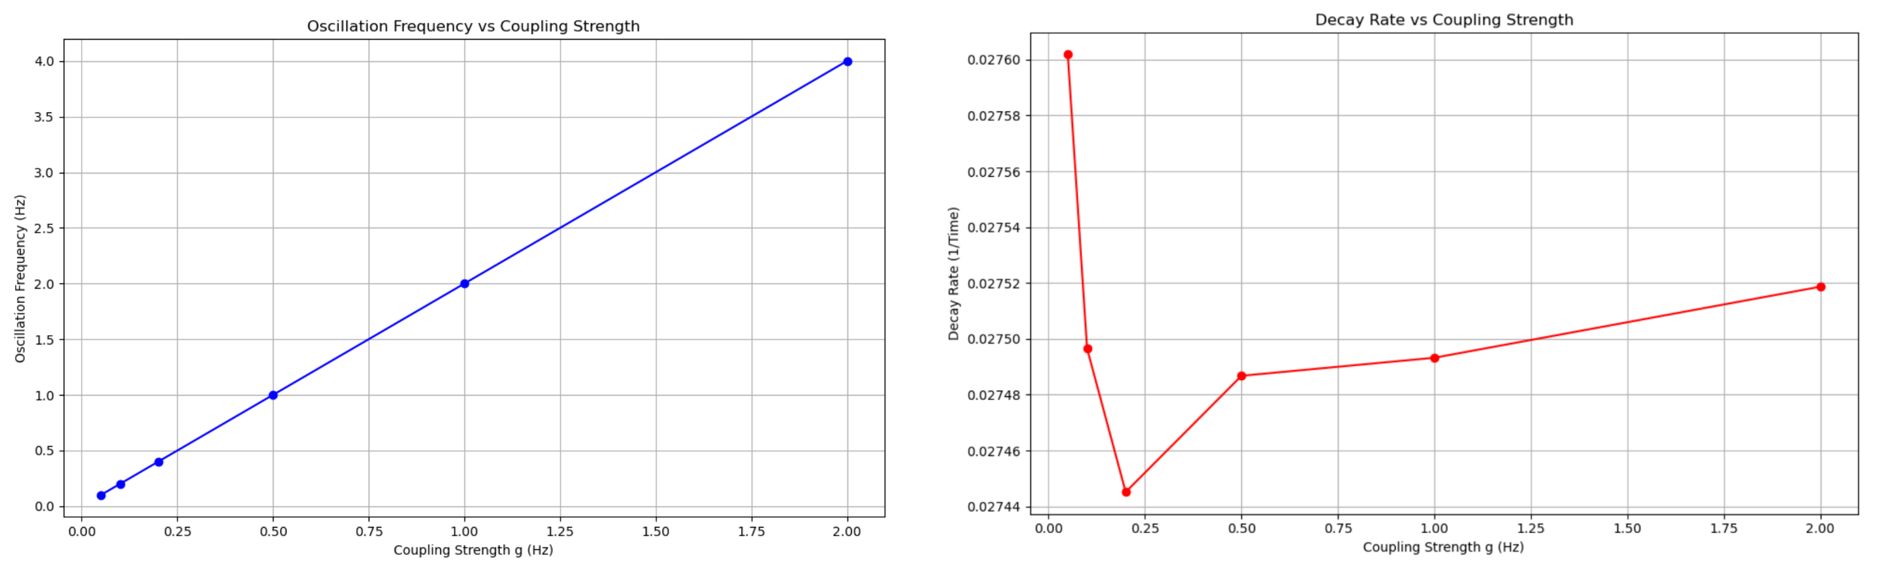
\includegraphics[width=0.8\linewidth]{2.png}
    \caption{Oscillation Frequency and Decay Rate vs. Coupling Strength. The left panel shows frequency vs. $g$, and the right panel shows decay rate vs. $g$.}
    \label{fig:frequency_decay}
\end{figure}

\subsection{Impact of Dissipation Rates on Rabi Oscillations}

Figure~\ref{fig:dissipation_rates} explores the effects of dissipation rates ($\kappa$ and $\gamma$) on the system's coherence. Higher dissipation rates lead to faster decay of oscillations, with $\kappa = 0.05$ and $\gamma = 0.05$ exhibiting rapid damping.

\begin{figure}[h!]
    \centering
    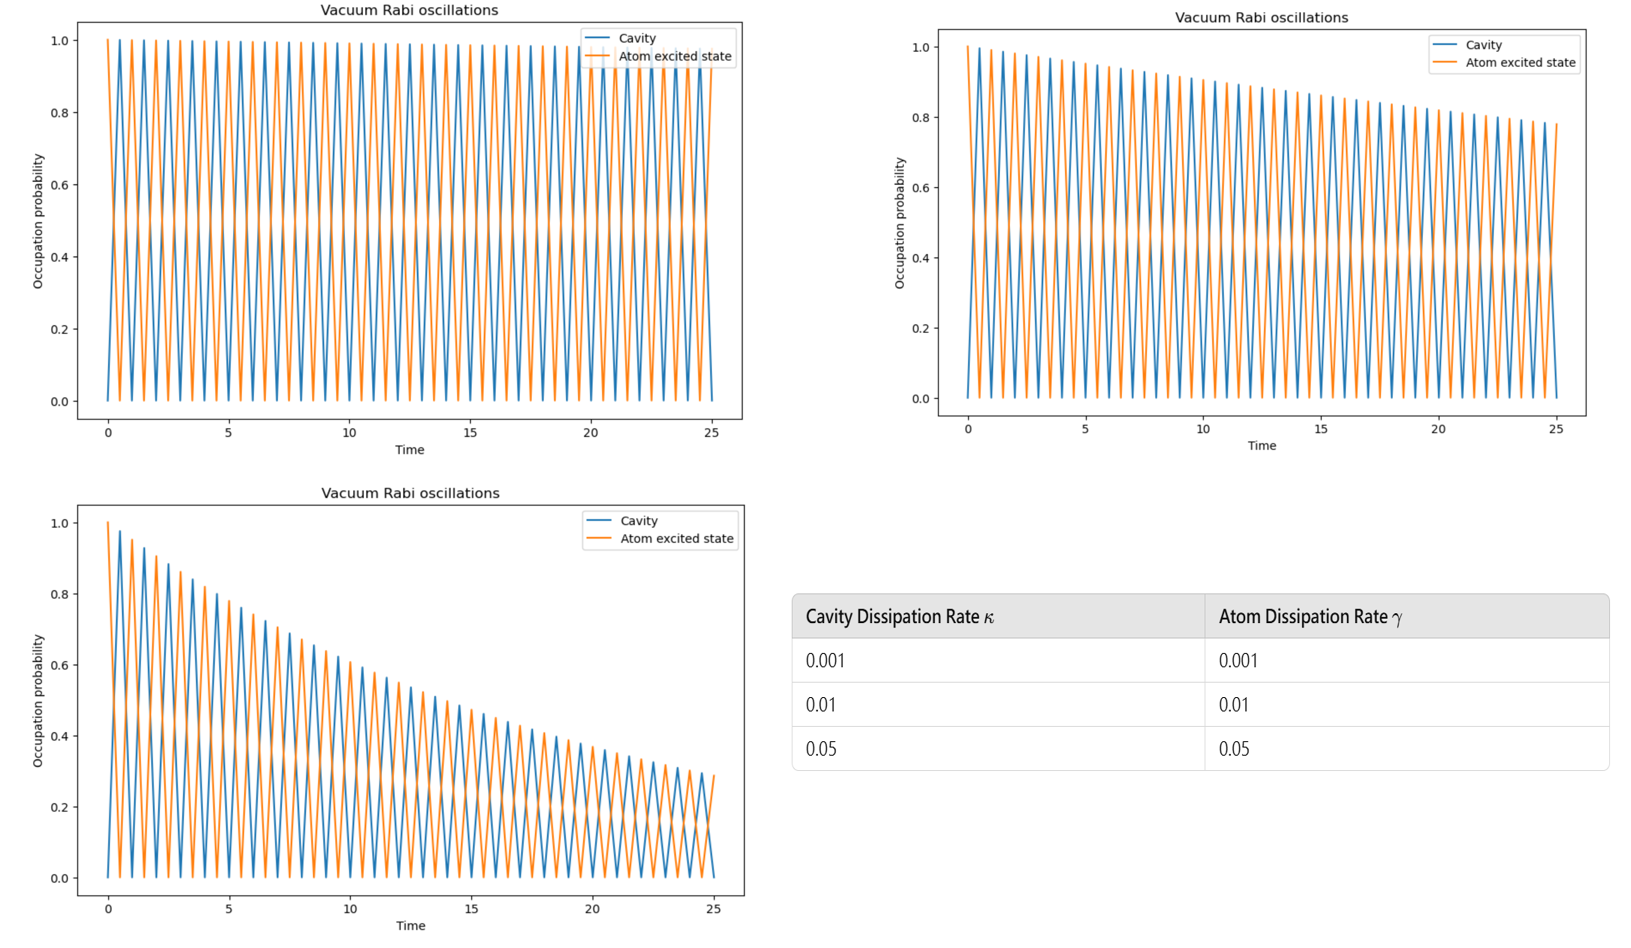
\includegraphics[width=0.8\linewidth]{3.png}
    \caption{Impact of Dissipation Rates on Vacuum Rabi Oscillations. Panels show the effects of increasing $\kappa$ and $\gamma$ on oscillatory coherence.}
    \label{fig:dissipation_rates}
\end{figure}

\subsection{Decay Rate vs. Dissipation Parameters}

Figure~\ref{fig:decay_vs_dissipation} shows a linear relationship between decay rates and dissipation parameters. Cavity dissipation ($\kappa$) exhibits a stronger influence compared to emitter dissipation ($\gamma$).

\begin{figure}[h!]
    \centering
    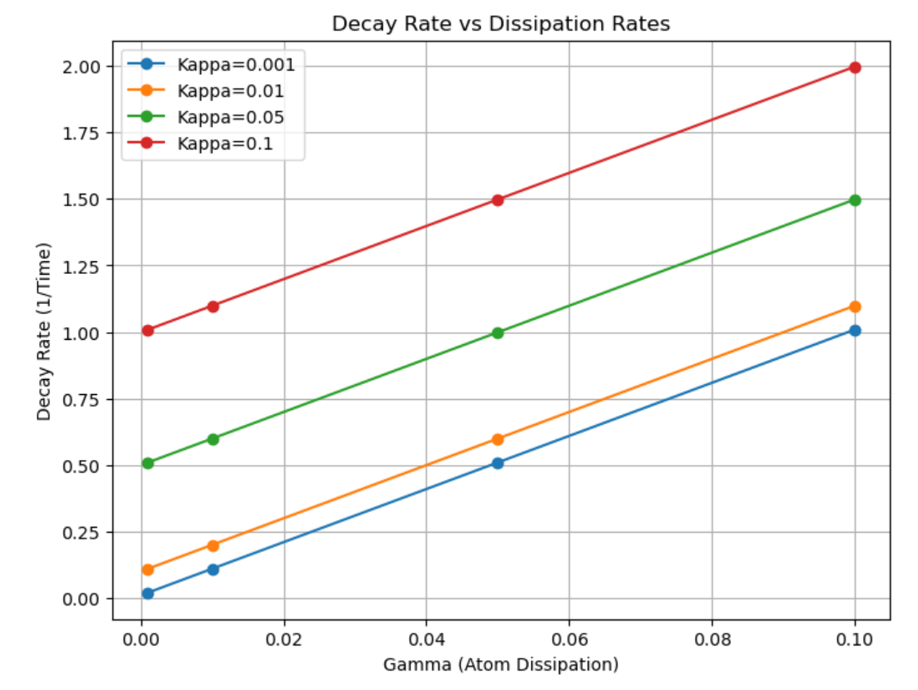
\includegraphics[width=0.8\linewidth]{4.png}
    \caption{Decay Rate vs. Dissipation Parameters. Linear trends show the effect of $\kappa$ and $\gamma$ on decay rates.}
    \label{fig:decay_vs_dissipation}
\end{figure}

\subsection{Effect of Thermal Noise on Rabi Oscillations}

The influence of thermal noise ($n_{\text{th}}$) is depicted in Figure~\ref{fig:thermal_noise}. Higher $n_{\text{th}}$ reduces oscillatory coherence and drives the system toward a thermal equilibrium state.

\begin{figure}[h!]
    \centering
    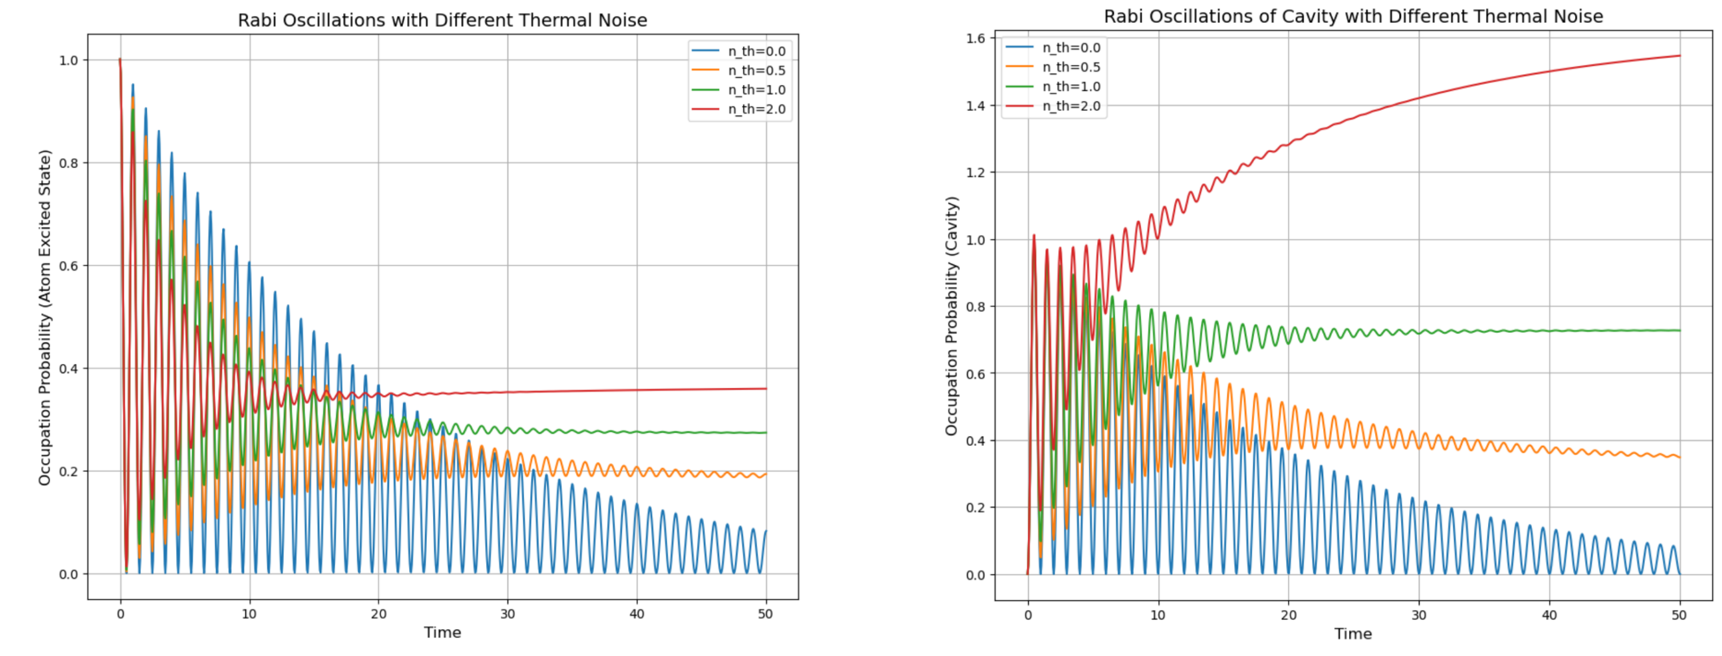
\includegraphics[width=0.8\linewidth]{5.png}
    \caption{Effect of Thermal Noise on Rabi Oscillations. Panels illustrate the impact of increasing $n_{\text{th}}$ on emitter and cavity populations.}
    \label{fig:thermal_noise}
\end{figure}

The figures collectively highlight the sensitivity of vacuum Rabi oscillations to system parameters and underscore the importance of precise control for quantum applications.

\section{Discussion}
The simulation results provide valuable insights into the dynamics of a single quantum emitter interacting with a single-mode cavity under various conditions. The analysis highlights several key phenomena:

\begin{itemize}
    \item \textbf{Impact of Coupling Strength ($g$):} As the coupling strength increases, the system transitions from weak to strong coupling regimes, leading to the emergence of pronounced Vacuum Rabi oscillations. This demonstrates the coherent energy exchange between the emitter and the cavity, which is fundamental to cavity quantum electrodynamics (CQED).
    \item \textbf{Effect of Dissipation Rates ($\kappa$ and $\gamma$):} Increasing dissipation rates suppresses Rabi oscillations, reflecting the decoherence introduced by cavity decay and emitter decay. These results emphasize the importance of minimizing loss mechanisms in experimental setups to maintain coherence and maximize the fidelity of quantum operations.
    \item \textbf{Thermal Noise ($n_{\text{th}}$):} The inclusion of thermal noise further degrades the coherence of the system. Higher noise levels lead to rapid damping of oscillations and a steady-state population imbalance, highlighting the challenges of maintaining quantum coherence in nonideal, high-temperature environments.
\end{itemize}



Building on these findings, several avenues for future exploration are proposed:

\begin{itemize}
    \item \textbf{Exploration of Multi-Emitter Systems:} Extending this analysis to systems involving multiple quantum emitters coupled to a single-mode cavity can provide insights into collective quantum phenomena, such as superradiance and subradiance. These systems are crucial for scalable quantum networks.
    \item \textbf{Incorporation of Dephasing and Complex Noise Models:} The current model considers dissipation and thermal noise, but does not include pure dephasing or correlated noise effects. Introducing such factors would offer a more realistic depiction of CQED systems, particularly in noisy environments.
    \item \textbf{Hybrid Quantum Systems:} Investigating hybrid platforms that integrate solid-state defects, such as T centers, with optical cavities can pave the way for practical quantum devices. Such studies could focus on optimizing coupling strength and coherence times in these platforms.
    \item \textbf{Advanced Cavity Designs:} Exploring novel photonic crystal cavity geometries or fiber-based Fabry-Pérot resonators with ultra-low loss could further reduce dissipation rates. These designs could enhance coherence and enable longer interaction times for advanced quantum operations.
    \item \textbf{Application in Quantum Technologies:} Applying these findings to practical implementations, such as quantum error correction codes or entanglement distribution in quantum communication systems, could bridge the gap between theory and real-world quantum technologies.
    \item \textbf{Integration with Machine Learning:} Utilizing machine learning techniques to optimize cavity and emitter parameters, predict system behavior, and mitigate decoherence offers a promising direction for achieving robust quantum operations in complex environments.
\end{itemize}

These future directions, combined with ongoing advances in experimental techniques, have the potential to significantly enhance our understanding of CQED systems and enable their deployment in next-generation quantum technologies.

\section*{Acknowledgements}
The author would like to thank Prof. Songtao Chen at the Department of Electrical and Computer Engineering at Rice University for their guidance and support throughout this project. Special thanks to the instructor of the ELEC 594 course for providing valuable feedback and resources that greatly contributed to the development of this work. Furthermore, the use of Python’s QuTiP library was instrumental in performing the numerical simulations presented in this paper. 

\section*{}

\begin{thebibliography}{99}
    \bibitem{Jaynes-Cummings} E. T. Jaynes and F. W. Cummings, ``Comparison of quantum and semiclassical radiation theories with application to the beam maser,'' \textit{Proceedings of the IEEE}, vol. 51, no. 1, pp. 89--109, 1963.
    
    \bibitem{QuTiP} J. R. Johansson, P. D. Nation, and F. Nori, ``QuTiP: An open-source Python framework for the dynamics of open quantum systems,'' \textit{Computer Physics Communications}, vol. 183, no. 8, pp. 1760--1772, 2012.

    \bibitem{Rabi} I. I. Rabi, ``On the process of space quantization,'' \textit{Physical Review}, vol. 49, no. 4, pp. 324--328, 1936.

    \bibitem{StrongCoupling} K. M. Birnbaum et al., ``Photon blockade in an optical cavity with one trapped atom,'' \textit{Nature}, vol. 436, no. 7047, pp. 87--90, 2005.

    \bibitem{HybridSystems} A. Sipahigil et al., ``An integrated diamond nanophotonics platform for quantum-optical networks,'' \textit{Science}, vol. 354, no. 6314, pp. 847--850, 2016.

    \bibitem{PhotonicCrystal} O. Painter et al., ``Two-dimensional photonic band-gap defect mode laser,'' \textit{Science}, vol. 284, no. 5421, pp. 1819--1821, 1999.

    \bibitem{ThermalNoise} F. Verstraete, M. M. Wolf, and J. I. Cirac, ``Quantum computation and quantum-state engineering driven by dissipation,'' \textit{Nature Physics}, vol. 5, no. 9, pp. 633--636, 2009.

    \bibitem{ErrorCorrection} A. Kitaev, ``Fault-tolerant quantum computation by anyons,'' \textit{Annals of Physics}, vol. 303, no. 1, pp. 2--30, 2003.

    \bibitem{MachineLearning} F. Biamonte et al., ``Quantum machine learning,'' \textit{Nature}, vol. 549, no. 7671, pp. 195--202, 2017.
\end{thebibliography}

\end{document}

